Aus den beobachteten Effekten Dunkler Materie lassen sich bereits Eigenschaften ableiten, welche von Teilchenkandidaten erfüllt sein müssen.
Dunkle Materie interagiert nur sehr schwach, ist stabil auf der kosmologischen Zeitskala und ist zum Großteil kalt (nicht relativistisch).
Die Liste möglicher Kandidaten ist zahlreich.
Von besonderem Interesse sind diejenigen, die zusätzlich aus anderen Teilgebieten der Physik motiviert sind.

\subsection*{Axion}
\acs{CP}-Verletzung sollte in der starken Wechselwirkung möglich sein, konnte bisher allerdings nicht beobachtet werden.
Die Abwesenheit von CP-Verletzung in der starken Wechselwirkung ist als starkes CP-Problem bekannt.
Durch das Hinzufügen einer $U(1)$ \ac{PQ} Symmetrie kann dieses gelöst werden.\cite{Peccey1977}
Das Axion ist das Nambu-Goldstone Boson der spontanen Brechung dieser Symmetrie.
Aufgrund stellarer Entwicklung wird erwartet, dass die Masse des Axions kleiner als $\SI{e-2}{\electronvolt}$\cite{Raffelt1999} ist.
Nicht thermische Axionen könnten trotzdem ein Kandidat für kalte DM sein.\cite{Drees2012}
Eine Auswahl verschiedener Ausschlussbereiche für die Axionmasse und die Kopplung an zwei Photonen ist in Abb. \ref{fig:AxionExclusion} gegeben.

\begin{figure}[!b]
\begin{center}
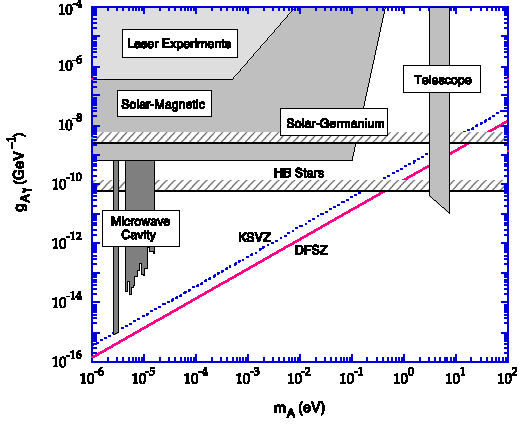
\includegraphics[width=0.8\textwidth]{./fig/AxionExclusion.pdf}
\end{center}
\vspace{-0.5cm}
\caption{Ausschlussbereiche der Axionmasse und Kopplung an zwei Photonen.
Auf der vertikalen Axe ist die effektive Kopplung des Axions an zwei Photonen aufgetragen und auf der horizontalen die Masse.
KSVZ und DSVZ sind zwei Klassen von Axion Modellen.
DM Axionen werden zwischen diesen Modellen im Massenbereich von $\SI{1}{\mu\electronvolt}\--\SI{100}{\mu\electronvolt}$ erwartet.\cite{Rosenberg2010}}
\label{fig:AxionExclusion}
\end{figure}

\subsection*{WIMPs}
Als WIMP (weakly interacting massive particles) wird eine Gruppe von Teilchen bezeichnet, welche eine Masse im Bereich von $\SI{10}{\giga\electronvolt}\--\SI{1}{\tera\electronvolt}$ haben und Wirkungsquerschnitte in der Größenordnung schwacher Wechselwirkungen\cite{Drees2012}.
WIMPs entstanden im frühen Universum im thermischen und chemischen Gleichgewicht mit Teilchen des \ac{SM}. 
Beim Abkühlen des Universums fällt die Anzahl der WIMPs ab einer Temperatur kleiner der WIMP Masse, aufgrund des Boltzmann-Faktors, exponentiell ab.
Da sich das Universum allerdings gleichzeitig ausdehnt kommt es ab dem Punkt an dem die Paarvernichtungsrate kleiner als die Expansionsrate des Universums ist, zum Freeze-out und die Teilchendichte bleibt nahezu konstant.
Es bleibt eine so genannte relic density übrig.
Liegt der Wirkungsquerschnitt für WIMPs in der Größenordnung schwacher Wechselwirkungen, ergibt sich für die relic density die aus kosmologischen Beobachtungen erwartete DM Dichte.
Dies wird als WIMP miracle bezeichnet.
Eigentlich motiviert als Lösung des gauge hirachy problem tauchen in der \ac{SUSY} mögliche WIMP Kandidaten auf.
SUSY ist eine Erweiterung des SM in dem eine Symmetrie zwischen Fermionen und Bosonen eingeführt wird.
Dies fordert weitere Teilchen welche sich im Spin um $1/2$ zu ihrem SM Partner unterscheiden.
Das leichteste supersymmetrische Teilchen ist aufgrund der neuen Erhaltungsgröße R-Parität stabil und daher ein möglicher WIMP Kandidat.
Dieses könnte das Neutralino sein.\cite{Feng2010}

%\subsection*{Sterile Neutrinos}

